% ----------------------------------------------------------------------
\begin{frame}{\gringo}
  \begin{itemize}
  \item \structure{Idea} \ systematically replace object variables by variable-free terms,
    applying stable-model preserving simplifications
  \item \structure{Features}
    \begin{itemize}
    \item expressive modeling language
    \item procedural attachments
    \item meta programming
    \end{itemize}
  \item \structure{Technology} \  semi-naive database evaluation
  \item \structure{References} \ \cite{kamsch21a}
  \end{itemize}
\end{frame}
% ----------------------------------------------------------------------

% ----------------------------------------------------------------------
\begin{frame}[fragile]{Example: Graph Coloring}
\begin{tikzpicture}[remember picture,overlay]
  \node[xshift=-3.5cm,yshift=-4.5cm] at (current page.north east){%
  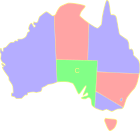
\includegraphics[width=.4\textwidth]{australia}};
\end{tikzpicture}
\begin{lstlisting}
% instance
vertex(a;b;c;d;e;f;g;h).
edge(a,(b;c)).
edge(b,(c;d)).
edge(c,(d;e;g)).
edge(d,e).
edge(e,(f;g)).
color(red;green;blue).

% encoding
{ assign(V,C) : color(C) } = 1 :- vertex(V).
:- edge(U,V), assign(U,C), assign(V,C).
\end{lstlisting}
\end{frame}
% ----------------------------------------------------------------------

% ----------------------------------------------------------------------
\begin{frame}[fragile,shrink=1]{Grounding}
\begin{lstlisting}
$ gringo --text enconding.lp instance.lp
vertex(a). vertex(b). vertex(c). vertex(d). vertex(e). vertex(f). vertex(g). vertex(h).
edge(a,b). edge(a,c). edge(b,c). edge(b,d). edge(c,d).
edge(c,e). edge(c,g). edge(d,e). edge(e,f). edge(e,g).
color(red). color(green). color(blue).
{ assign(a,red); assign(a,green); assign(a,blue)} = 1.
{ assign(b,red); assign(b,green); assign(b,blue)} = 1.
{ assign(c,red); assign(c,green); assign(c,blue)} = 1.
{ assign(d,red); assign(d,green); assign(d,blue)} = 1.
{ assign(e,red); assign(e,green); assign(e,blue)} = 1.
{ assign(f,red); assign(f,green); assign(f,blue)} = 1.
{ assign(g,red); assign(g,green); assign(g,blue)} = 1.
{ assign(h,red); assign(h,green); assign(h,blue)} = 1.
:- assign(b,red),assign(a,red).     :- assign(b,green),assign(a,green).
:- assign(b,blue),assign(a,blue).   :- assign(c,red),assign(a,red).
:- assign(c,green),assign(a,green). :- assign(c,blue),assign(a,blue).
:- assign(c,red),assign(b,red).     :- assign(c,green),assign(b,green).
:- assign(c,blue),assign(b,blue).   :- assign(d,red),assign(b,red).
:- assign(d,green),assign(b,green). :- assign(d,blue),assign(b,blue).
:- assign(d,red),assign(c,red).     :- assign(d,green),assign(c,green).
:- assign(d,blue),assign(c,blue).   :- assign(e,red),assign(c,red).
:- assign(e,green),assign(c,green). :- assign(e,blue),assign(c,blue).
:- assign(g,red),assign(c,red).     :- assign(g,green),assign(c,green).
:- assign(g,blue),assign(c,blue).   :- assign(e,red),assign(d,red).
:- assign(e,green),assign(d,green). :- assign(e,blue),assign(d,blue).
:- assign(f,red),assign(e,red).     :- assign(f,green),assign(e,green).
:- assign(f,blue),assign(e,blue).   :- assign(g,red),assign(e,red).
:- assign(g,green),assign(e,green). :- assign(g,blue),assign(e,blue).
\end{lstlisting}
\end{frame}
% ----------------------------------------------------------------------

% ----------------------------------------------------------------------
\begin{frame}[fragile,shrink=1]{Grounding for the Solver}
\begin{lstlisting}
$ gringo enconding.lp instance.lp
asp 1 0 0
1 0 1 1 0 0
1 0 1 2 0 0
...
1 0 0 0 2 30 31
1 0 0 0 2 32 33
...
1 1 3 31 33 35 0 1 22
1 0 1 51 1 1 3 31 1 33 1 35 1
1 0 1 52 1 2 3 31 1 33 1 35 1
1 0 1 53 0 2 51 -52
1 0 0 0 2 22 -53
...
4 10 color(red) 0
4 12 color(green) 0
...
4 13 assign(a,red) 1 31
4 13 assign(b,red) 1 30
...
4 9 vertex(a) 0
4 9 vertex(b) 0
...
4 9 edge(a,b) 0
4 9 edge(a,c) 0
...
0
\end{lstlisting}
\end{frame}
% ----------------------------------------------------------------------

%%% Local Variables:
%%% mode: latex
%%% TeX-master: "../../main"
%%% End:
